
\section{Introduction}

In recent years, deep neural networks have become state-of-the-art solutions for many tasks. However, for some, they tend to achieve high overall prediction accuracy at the cost of mispredicting samples from minority groups. This is dangerous for automatic decision systems that make critical decisions. For instance, models trained with Empirical Risk Minimization (\texttt{ERM}) are particularly susceptible to this issue. One of the key reasons for this behavior, identified by both \citet{sagawa2020distributionally} and \citet{koh2021wilds}, is the existence of spurious correlations between the features and labels of the majority group, which may not exist or correlate negatively for minority groups. To overcome this, several new algorithms have been proposed, such as Group Distributionally Robust Optimization (\texttt{Group‐DRO} or \texttt{G-DRO}) \cite{sagawa2020distributionally}, and Common Gradient Descent (\texttt{CGD}) \cite{piratla2022focus}. The first tackles the problem by training on the group with the largest training loss. Nevertheless, \citet{piratla2022focus} observed that this might lead to imbalanced training due to increased loss in the other groups. In contrast, \texttt{CGD} trains on the group which minimizes the loss across all groups. The authors claim that such an approach models inter-group interactions and addresses spurious correlations. This report aims to verify the claims of the authors by reproducing their findings and performing additional experiments. Our contribution can be summarized as follows:

\begin{itemize}
    \item We reproduce both the qualitative and quantitative experiments to identify which claims can be verified. We also quantify the computational and development cost needed.
    \item We update the \texttt{CGD} code to make it compatible with the latest version of the WILDS framework \cite{koh2021wilds} and document the steps taken to reproduce the paper, making future reproductions easier and more accessible.
    \item We implemented the code required to run experiments on the MultiNLI \cite{williams2018broad} dataset.
\end{itemize}


\section{Scope of reproducibility}
\label{sec:claims}

The paper ``Focus On The Common Good: Group Distributional Robustness Follows'' \cite{piratla2022focus} attempts to tackle the problems of spurious correlations and sub-population shift with a new optimization algorithm: Common Gradient Descent (\texttt{CGD}). \texttt{CGD} optimizes the model using the group ``whose gradients lead to the largest decrease in average training loss over all groups'' \cite{piratla2022focus}. In this reproducibility study, we attempt to validate the following claims made by the authors:


\begin{itemize}
    \item \texttt{CGD} is more robust than \texttt{Group-DRO} in the presence of spurious features: by focusing on the group that leads to the largest loss decrease across all groups, \texttt{CGD} is robust against spurious features.
    \item \texttt{CGD} generalizes better across all groups in comparison to \texttt{ERM}: a model trained with \texttt{CGD} should perform better on minority groups while achieving a comparable average accuracy.
    \item \texttt{CGD} monotonically decreases the macro/group-average loss: the authors prove this claim mathematically, showing that \texttt{CGD} finds first-order stationary points. We attempt to validate this claim empirically over three datasets used by the paper.
\end{itemize}

In this reproducibility study, due to resource and time constraints, we decided to compare the performance of \texttt{CGD} only against \texttt{ERM} and \texttt{Group-DRO}. This decision is also motivated by the fact that the other robustness algorithms mentioned in the paper were not discussed as thoroughly. We consider this subset of algorithms sufficient to validate the claims stated above. Moreover, for the real-world datasets from the WILDS benchmark \cite{koh2021wilds}, we only trained with \texttt{CGD}, given that the documented results with the other algorithms were highly correlated with the values reported in the official WILDS paper \cite{koh2021wilds} and the WILDS benchmark. Therefore, we felt these two were reliable sources for validating these results.


\section{Methodology}

To conduct our experiments we utilized the code for \texttt{CGD} which was released by the authors on their GitHub repository \footnote{\url{https://github.com/vihari/CGD}}. The available implementation was designed to be run using version 1.2.2 of the WILDS framework \cite{koh2021wilds}. In the months following the code release, WILDS underwent a major update \cite{sagawa2021extending} to version 2.0. In order to make \texttt{CGD} compatible with the new framework version, we had to implement some minor tweaks, especially for datasets with disjoint groups for the training, validation, and test sets. The authors also provided the initialization code for the datasets used in the qualitative evaluation of the algorithm. The code for the datasets used in the quantitative evaluation was included in the WILDS repository, except for MultiNLI, which we implemented using the code in the \texttt{Group-DRO} repository \cite{sagawa2020distributionally} as indicated by the authors.


\subsection{Algorithm descriptions}

This section describes the algorithms used to validate the claims made by the authors, namely \texttt{ERM}, \texttt{Group-DRO}, and \texttt{CGD}. We closely follow the notation used in the paper, which defines $\mathcal{X}$, $\mathcal{Y}$ as the feature and label spaces, and $\mathcal{G}$ as a set of non-overlapping $k$ groups, each composed of $n_i$ observations distributed as $P_i(\mathcal{X}, \mathcal{Y})$. For each group $i$, we define $\ell_i(\theta) = \mathbb{E}_{(x, y)\sim P_i(\mathcal{X}, \mathcal{Y})}\mathcal{L}(x, y; f_\theta)$ as group loss, where $f_\theta$ is a classifier, $\theta$ are the model parameters and $\mathcal{L}$ is an appropriate loss. The baseline algorithm is \texttt{ERM}, which minimizes the expected training loss.

\begin{equation}
\begin{aligned}[c]
\theta^{t+1}_{\texttt{ERM}} = \underset{\theta}{\text{argmin }} \{\mathbb{E}_{(x, y)\sim \hat{P}}[\ell(\theta^t)]\} \text{ ,}
\end{aligned}
\label{eq:ERM_algo}
\end{equation}


where $\hat{P}$ is the empirical distribution over the training data and $\ell$ the loss for the whole training set without considering the groups. The \texttt{ERM} formulation implicitly assigns a higher weight to majority groups. It also encourages the model to exploit spurious correlations that work well for predicting the label of majority groups, achieving high average test accuracies at the expense of minority groups. To overcome this issue, \citet{sagawa2020distributionally} proposed \texttt{Group-DRO}, which, at each step, trains on the group with the worst training loss $j^*$:

\begin{equation}
\begin{aligned}[c]
j^* = \underset{i\in \mathcal{G}}{\text{argmax }}{\ell_i (\theta)}
\end{aligned}
\qquad\Rightarrow\qquad
\begin{aligned}[c]
\theta^{t+1}_{\texttt{G-DRO}} = \theta^t-\eta\nabla \ell_{j^*}(\theta^t)
\end{aligned}
\label{eq:gdro_algo}
\end{equation}


While \texttt{Group-DRO} has a better performance on minority groups when compared to \texttt{ERM}, it may overfit on them, jeopardizing the average loss over all groups. To solve this problem, \citet{piratla2022focus} proposed Common Gradient Descent (\texttt{CGD}), which, at each step, picks the group which minimizes the overall loss across all groups as follows:


\begin{equation}
\begin{aligned}[c]
j^* = \underset{j}{\text{argmin}}\{\sum_i\ell_i[\theta^t-\eta\nabla_{\theta}\ell_{j}(\theta^t)]\}
\end{aligned}
\qquad\Rightarrow\qquad
\begin{aligned}[c]
\theta^{t+1}_{\texttt{CGD}} = \theta^t-\eta\sum_i{\alpha_i^{t+1}}\nabla_{\theta}\ell_{i}(\theta^t) \text{ ,}
\end{aligned}
\label{eq:cgd_algo}
\end{equation}

where $\alpha_i$ is the weight for group $i$. A more thorough explanation of this formula and the \texttt{CGD} algorithm is provided in the original paper. The algorithms above were evaluated on various model/dataset combinations as shown in Table \ref{tab:models} of Appendix \ref{appendix:Model}.

\subsection{Datasets}
\label{sec:datasets}

The paper uses two groups of datasets: one composed of 2 synthetic toy datasets to compare the qualitative performance of \texttt{CGD} against \texttt{Group-DRO}, and a second one consisting of 2 synthetic datasets and six real-world datasets.

% \subsubsection{Qualitative Evaluation} The qualitative performance of \texttt{CGD} was evaluated on two toy datasets with three multi-group setups: {Simple}, a 2-feature dataset sampled from a standard normal distribution, and {MNIST}. The three setups, each with three groups, are {Noisy}, where 20\% of the first group labels were flipped for {Simple} and 50\% for {MNIST}. {Rotation}, where labels (or the images for {MNIST}) were rotated by 30 degrees per group, such that the optimal classifier is the optimal classifier of the second group and {Spurious}, where each sample has a third feature (the digit color for MNIST), which has an 80\% correlation with the label.

\subsubsection{Qualitative Evaluation} The qualitative performance of \texttt{CGD} was evaluated on two toy datasets: a 2-feature dataset sampled from a standard normal distribution, and {MNIST}. On these datasets we applied three multi-group setups:
\begin{itemize}
    \item Label Noise Setup - where 20\% of the first group labels were flipped for Simple and 50\% for MNIST.
    \item Rotation Setup - where labels (or the images for MNIST) were rotated by 30 degrees per group, such that the distances from the first and third group to the second is the same.
    \item Spurious Setup - where each sample has a third feature (the digit color for MNIST), which has an 80\% correlation with the label.
\end{itemize}


\subsubsection{Quantitative Evaluation}
For the quantitative evaluation of the algorithm, we used eight datasets categorized into synthetic or real-world and based on whether they include spurious correlations (non-WILDS) or sub-population shift (WILDS). The datasets are summarized in Table \ref{tab:all-datasets-summary}.

\begin{table}[h]
\centering
\begin{threeparttable}
\begin{tabular}{lcll}\toprule
    \textbf{Dataset (non-WILDS)} & \textbf{Type} & \textbf{Classes} & \textbf{Spurious Variable} \\
    \midrule
    CMNIST \cite{gulrajani2021search} & S & Digits & Digit Color \\
    WaterBirds \cite{sagawa2020distributionally} & S & Water/landbird & Background \\
    CelebA \cite{liu2015deep} & R & Blond/Non-Blond & Gender \\
    MultiNLI \cite{williams2018broad} & R & NLI\tnote{a} & Negation Words \\
    \midrule
    \textbf{Dataset (WILDS)} & \textbf{Type} & \textbf{Classes} & \textbf{Groups} \\
    \midrule
    Camelyon17 \cite{bandi2019detection} & R & Tumor/Non-Tumor & Source Hospital \\
    PovertyMap \cite{yeh2020using} & R & Wealth-Index & Country \& Rural/Urban \\
    FMoW \cite{christie2018functional} & R & Building/Land use & Year \& Region \\
    CivilComments \cite{borkan2019nuanced} & R & Toxic/Non-Toxic & Mentioned Demographics\\
    \bottomrule
\end{tabular}
\begin{tablenotes}\footnotesize
\item [a] Natural Language Inference
\end{tablenotes}
\caption{Summary of the datasets used for the quantitative evaluation. Datasets are categorized into synthetic (S) or real (R) and based on whether they include spurious correlations (non-WILDS) or sub-population shift (WILDS). The rightmost column shows the spurious variable for the non-WILDS dataset and the groups in which samples are partitioned for the WILDS datasets. MultiNLI and CivilComments are text datasets, while the others are image datasets.}
\label{tab:all-datasets-summary}
\end{threeparttable}
\end{table}

\subsection{Hyperparameters}
\label{sec:hypparam}
% Describe how the hyperparameter values were set. If there was a hyperparameter search done, be sure to include the range of hyperparameters searched over, the method used to search (e.g. manual search, random search, Bayesian optimization, etc.), and the best hyperparameters found. Include the number of total experiments (e.g. hyperparameter trials). You can also include all results from that search (not just the best-found results).

\begin{table}
\centering
\begin{tabular}{lrrrrrrr}\toprule
    \textbf{Dataset} & \textbf{lr} & \textbf{Weight Decay} & \textbf{Epochs} & \textbf{Batch Size} & \textbf{C} & \textbf{Step Size} \\\midrule
CMNIST & 1e-3 & 1e-1 & 10 & 32 & 0 & 0.05 \\
WaterBirds & 1e-3 & 1e-1 & 300 & 128 & 2 & 0.05 \\
CelebA & 1e-3 & 1e-4 & 10 & 8 & 2 & 0.05 \\
MultiNLI & 1e-3 & 1e-4 & 3 & 8 & 2 & 0.05 \\
CivilComments & 1e-5 & 1e-2 & 5 & 16 & 0 & 0.05 \\
PovertyMap & 1e-3 & 0 & 10 & 64 & 0 & 0.05 \\
FMoW & 1e-4 & 0 & 5 & 32 & 0 & 0.2 \\
Camelyon17 & 1e-3 & 1e-2 & 5 & 32 & 0 & 0.05\\\bottomrule

\end{tabular}
\caption{Hyperparameters used for each dataset and all algorithms in our experiments. C and step size are only relevant for \texttt{CGD}. If a hyperparameter is not included then the default value in WILDS should be assumed.}
\label{tab:hyps}
\end{table}

\subsubsection{Qualitative Evaluation} the models for the qualitative evaluation are trained using SGD for 400 epochs, with a learning rate of 0.1 as indicated in the paper. The batch size and the weight decay are not specified, and we used respectively 128 and 0.01, the latter of which was selected from the set $\{1, 0.1, 0.01, 0.001, 0\}$ by manually inspecting the \texttt{CGD} training weights ($\alpha$) plots and choosing the value which produces a plot resembling Figure 1 of the original paper.

\subsubsection{Quantitative Evaluation} following \citet{piratla2022focus} the models for the qualitative evaluation are trained using SGD with a momentum of 0.9, except for PovertyMap, which uses Adam. For the WILDS datasets, we followed the setup in \citet{koh2021wilds}, with some exceptions for the number of epochs and the batch size due to computational limitations. For \texttt{CGD}, the group-adjustment parameter $C$ is 0 following \citet{piratla2022focus} and the step size $\eta$ is selected from the WILDS leaderboard\footnote{\url{https://wilds.stanford.edu/leaderboard/}}. As for the non-WILDS datasets, the authors ran a grid search over the learning rate, weight decay, batch size, and $C$ (set to 0 for CMNIST), but only provided the hyperparameter ranges and not the selected values. Due to computational constraints, we used the values provided in the \texttt{Group-DRO} paper \cite{sagawa2020distributionally}, but if the value was out of the range defined by the authors, we selected the closest one in that range. For \texttt{CGD}, $C$ was set to 2 according to \citet{sagawa2020distributionally}, and $\eta$ according to the WILDS leaderboard. The hyperparameter values are summarized in Table \ref{tab:hyps}. The sensitivity of \texttt{CGD} with regards to hyperparameters $C$ and $\eta$ is explored in Appendix \ref{appendix:hyps-sensitivity}.

\subsection{Experimental setup and code}

To make our study reproducible, we provide a guide on setting up a conda environment with all the required dependencies in our GitHub repository. The instructions are for a Google Compute Engine (GCE) virtual machine with preinstalled NVIDIA drivers. However, they are highly flexible and should work on any machine with minor tweaks (namely the CUDA version). We also provide a modified version of the WILDS repository which can run the \texttt{CGD} experiments out of the box. The complete instructions on reproducing our experiments are available in the README.md file of the repository.


\subsection{Computational requirements}

The experiments were executed on three machines, whose hardware configurations are listed in Table \ref{tab:machines}. The estimated runtime of each model/dataset pair on a Google Compute Engine Virtual Machine (GCE) is listed in Table \ref{tab:algo-runtimes}, and each pair was run with three different seeds. Therefore the total computation time was approximately 440 hours.


\begin{table}[h]
    \centering
    \begin{tabular}{llrlr}\toprule
        \textbf{Machine} & \textbf{CPU} & \textbf{RAM (GB)} & \textbf{Graphics Card} & \textbf{VRAM (GB)} \\\midrule
        GCE VM & Intel Xeon 8173M & 16 & Tesla T4  & 16\\
        Laptop A & AMD Ryzen 7 5800h & 16 & RTX 3050Ti Mobile & 4\\
        Laptop B & Intel i5‐9300H & 16 & GTX 1660Ti Mobile  & 6\\
        \bottomrule
    \end{tabular}
    \caption{Hardware configuration of the machines used to run experiments.}
    \label{tab:machines}
\end{table}

\vspace{-8pt}

\begin{table}[h]
    \centering
    \begin{tabular}{lrrrr}\toprule
        \textbf{Algorithm} & \textbf{CMNIST} & \textbf{WaterBirds} & \textbf{CelebA} & \textbf{MultiNLI} \\
        \midrule
        \texttt{ERM}, \texttt{Group-DRO} & 1h & 7h & 8h & 4h \\
        \texttt{CGD} & 2h & 15h & 31h & 4.5h \\
        \midrule
        \textbf{Algorithm} & \textbf{CivilComments} & \textbf{PovertyMap} &
        \textbf{FMoW} & \textbf{Camelyon17} \\
        \midrule
        \texttt{ERM}, \texttt{Group-DRO} & 16h & 0.3h & 2h & 3h \\
        \texttt{CGD} & 17h & 8h & 20h & 10h \\
        \bottomrule
    \end{tabular}
    \caption{Estimated runtime in hours of each model and dataset combination on a Google Compute Engine Virtual Machine with a Tesla T4 GPU. The runtimes of \texttt{ERM} and \texttt{Group-DRO} are similar for all datasets.}
    \label{tab:algo-runtimes}
\end{table}


\section{Results}
\label{sec:results}

\subsection{Results reproducing original paper}


\subsubsection{Qualitative Evaluation}

We replicated the qualitative comparison in Section 4 of the paper for both the Simple and MNIST datasets. For the Simple dataset, \texttt{CGD} outperforms \texttt{Group-DRO}, albeit with a smaller gap than the results of the paper, as can be seen in Table \ref{tab:qual-simple}. An inspection of the group weights $\alpha$ over epochs as shown in Figure \ref{fig:qualitative_exp} reveals the \texttt{CGD} effectively behaves as described in the paper:

\begin{itemize}
    \item Label Noise setup - \texttt{CGD} avoids training only on the noisy majority. 
    \item Rotation Setup - \texttt{CGD}, on average, focuses on the center group, which has the optimal classifier. However, this selection varies from seed to seed (Appendix \ref{appendix:qualitative_group_sel}).
    \item Spurious Setup - \texttt{CGD} correctly identifies the clean majority and assigns it a much stronger weight than in the paper.
\end{itemize}

% Figure \ref{fig:qualitative_exp}, where we plot the group weights and averaged them over six seeds, corroborates the claims. Just like in the original paper:

 For the MNIST dataset, we were not able to replicate the paper results. As shown in Table \ref{tab:qual-mnist}, we achieved similar average and worst-group accuracies between \texttt{CGD} and \texttt{Group-DRO}, except for the Rotation setup, where \texttt{Group-DRO} failed to achieve reasonable accuracy. We suspect there might be an issue with the experimental setup for \texttt{Group-DRO} because the original paper achieved significantly better results.

\begin{figure}[H]
    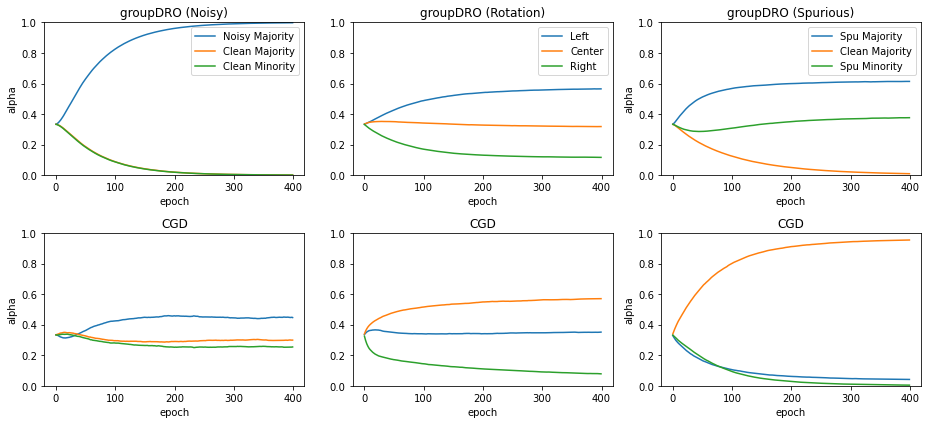
\includegraphics[width=\textwidth]{media/averaged-qualitative-plots-v2.png}
    \centering
    \caption{The comparison of group weights $\alpha$ for \texttt{Group-DRO} (top) and \texttt{CGD} (bottom) for the Simple dataset setups: label noise, rotation and spurious.}
    \label{fig:qualitative_exp}
\end{figure}

\begin{table}[H]
    \centering
    \begin{tabular}{lccc}
        \toprule
        \textbf{Algorithm} & \textbf{Noisy Simple} & \textbf{Rotation Simple} & \textbf{Spurious Simple} \\ 
        \midrule
        \texttt{G-DRO} & 0.26 (0.02) & 0.47 (0.04) & 0.42 (0.03) \\
        \texttt{CGD} & \textbf{0.22 (0.01)}	& \textbf{0.46 (0.06)} & \textbf{0.32 (0.01)} \\
    \bottomrule
    \end{tabular}
    \caption{Worst group losses on the test split of the simple dataset, averaged over six seeds. The standard deviation is shown in parentheses.}
    \label{tab:qual-simple}
\end{table}

\begin{table}[h!]
    \centering
    \begin{tabular}{llccc}
        \toprule
        \textbf{Algorithm} & \textbf{Metric} & \textbf{Noisy MNIST} & \textbf{Rotation MNIST} & \textbf{Spurious MNIST} \\ 
        \midrule
        \texttt{G-DRO} & Avg. Acc. & \textbf{77.36 (10.02)} & 30.58 (3.82) & \textbf{92.47 (2.63)} \\
        & W.g. Acc. & \textbf{77.25 (9.95)} & 28.02 (4.42) & \textbf{91.75 (2.68)} \\
        \texttt{CGD} & Avg. Acc. & 76.35 (7.8) & \textbf{92.51 (1.78)} & 92.51 (1.78) \\
        & W.g. Acc. & 76.24 (7.81) & \textbf{91.7 (2.35)} & 91.7 (2.35) \\
    \bottomrule
    \end{tabular}
    \caption{Average and worst group accuracies on the test split of MNIST, averaged over three seeds. The standard deviation is shown in parentheses.}
    \label{tab:qual-mnist}
\end{table}

\vspace{-8pt}

\subsubsection{Quantitative Evaluation} We reproduced the experiments on the non-WILDS and WILDS datasets and compared the performance of \texttt{CGD} against \texttt{ERM} and \texttt{Group-DRO}. Table \ref{tab:non_wilds_results} summarizes the results on the four non-WILDS datasets. \texttt{CGD} outperforms the other algorithms on the synthetic datasets with spurious correlations (CMNIST and WaterBirds), but fails to improve in the real-world datasets with spurious correlations (CelebA and {MultiNLI) over \texttt{ERM} and \texttt{Group-DRO}. As for the WILDS datasets whose results are shown in Table \ref{tab:wild_results}, \texttt{CGD} is the best algorithm only on Camelyon17 (albeit with a larger standard deviation than \texttt{ERM}) and on the in-domain evaluation of PovertyMap, while \texttt{ERM} has a significant advantage on the out-of-domain evaluation against \texttt{CGD}, showing a larger gap than what claimed by the paper. Overall, the results are in line with the paper, which shows that \texttt{CGD} is better in some setups and achieves comparable performances in others, but its superiority is not clear.


\begin{table}[H]
\centering
\begin{tabular}{lcccc} \\ \toprule
    & \multicolumn{2}{c@{\quad}}{\textbf{CMNIST}}
    & \multicolumn{2}{c@{\quad}}{\textbf{WaterBirds}}
    \\ \cmidrule(r){2-3} \cmidrule(l){4-5}  
\textbf{Algorithm}& Avg. Acc. & W.g. Acc. & Avg. Acc. & W.g. Acc.    \\ \midrule
\texttt{ERM} & 55.3  (2.23) & 10.5 (4.47) & 97.1 (0.03) & 52.2 (1.18)   \\
\texttt{G-DRO} & \textbf{97.6} (0.49) & \textbf{96.8} (0.69) & \textbf{97.3} (0.06) & 71.7 (0.55)   \\
\texttt{CGD} & \textbf{98.0} (0.34) & \textbf{97.0} (0.4) & \textbf{97.3} (0.13) & \textbf{73.2} (0.39)  \\ \bottomrule
\end{tabular}

\begin{tabular}{lcccc} \\ \toprule
    & \multicolumn{2}{c@{\quad}}{\textbf{CelebA}}
    & \multicolumn{2}{c@{\quad}}{\textbf{MultiNLI}}
    \\ \cmidrule(r){2-3} \cmidrule(l){4-5}  
\textbf{Algorithm}& Avg. Acc. & W.g. Acc. & Avg. Acc. & W.g. Acc.    \\ \midrule
\texttt{ERM} & \textbf{96.0} (0.12) & 36.3 (6.04) & \textbf{62.2} (11.27) & 16.1 (18.59)   \\
\texttt{G-DRO} & 94.9 (0.11) & 59.1 (1.72) & 49.9 (0.76) & \textbf{27.5} (2.62)  \\
\texttt{CGD}& 95.0 (0.13) & \textbf{59.8} (8.72) & 50.2 (1.01) & 27.1 (1.36) \\ \bottomrule

\end{tabular}
\caption{Average and worst-group accuracies on the test splits of the non-WILDS datasets. In parentheses are the standard deviations.}
\label{tab:non_wilds_results}
\end{table}


\begin{table}[H]
\centering
\begin{tabular}{lccccc} \\ \toprule
& \multicolumn{1}{c}{\textbf{Camelyon17}}
& \multicolumn{2}{c@{\quad}}{\textbf{PovertyMap}}
& \multicolumn{1}{c}{\textbf{FMoW} }
& \multicolumn{1}{c}{\textbf{CivilComments}} \\
& \multicolumn{1}{c}{Avg. Acc.}
& \multicolumn{2}{c@{\quad}}{{W.r. Pearson R}}
& \multicolumn{1}{c}{W.r. Acc.} 
& \multicolumn{1}{c}{W.g. Acc.} \\ 
 \cmidrule(l){2-2}
 \cmidrule(l){3-4}
 \cmidrule(l){5-5}
 \cmidrule(l){6-6}
\textbf{Algorithm} &
\multicolumn{1}{c}{OOD} &
\multicolumn{1}{c}{ID}  &
\multicolumn{1}{c}{OOD}  & \multicolumn{1}{c}{OOD} & \multicolumn{1}{c}{ID}
 \\\midrule
\texttt{ERM} & 70.3 (6.4) & 0.57 (0.07) & \textbf{0.45} (0.06) & \textbf{32.3} (1.2) &56.0 (3.6)\\
\texttt{G-DRO} & 68.4 (7.3)  & 0.54 (0.11) & 0.39 (0.06) & 30.8 (0.8) & \textbf{70.0} (2.0) \\
\texttt{CGD} & \textbf{70.4} (7.56) & \textbf{0.63} (0.03) & 0.38 (0.07) & 29.8 (1.46)	& 69.7 (1.09) \\\bottomrule

\end{tabular}
\caption{Results for different metrics on the test splits of the WILDS datasets. In parentheses are the standard deviations. w.r. and w.g stand for worst region and worst group accuracy. The values were taken from the original paper with the exception of \texttt{CGD} which we trained ourselves.}
\label{tab:wild_results}
\end{table}

\subsection{Results beyond original paper}

% As we can see from Table \ref{tab:algo-runtimes} there are some datasets for which the increase in runtime is more significant (for WaterBirds we have an increase of 50\%, while for the PovertyMap the increase if of 2000\%). We found that a reason for this was the need to compute the gradient of the losses for all groups (equation \ref{eq:cgd_algo}), to find what was the model weight update that would represent the minimum sum of losses in the next time step. To support this hypothesis, one could observe that the bigger increases in runtime comes from  PovertyMap, FMoW and Camelyon, that have 13, 16 and 5 groups, respectively, whereas the other groups do not have more than 4 groups. CelebA is an exception for this theory, but we believe that the increase in the runtime is due to the small batch size (8).

The paper does not discuss the runtime of the algorithms, which we documented in Table \ref{tab:algo-runtimes}. We find that \texttt{CGD} is often 2 to 26 times slower than the other algorithms depending on the dataset. As seen in Table \ref{tab:algo-runtimes}, the runtime increase varies across datasets: for WaterBirds, we have an increase of 50\%, while for PovertyMap, the increase is over 2000\%. The computation of the gradients for each group at each training step (Equation \ref{eq:cgd_algo}) might be one possible reason. This hypothesis is supported by the fact that datasets with many groups, such as PovertyMap, FMoW, and Camelyon, with 13, 16, and 5 groups respectively, had the largest increase in training time (the other datasets do not have more than four groups). CelebA is an exception, but the runtime increase may be due to the small batch size (8). In view of the above, we concluded that the small gains in accuracy may not justify the increased training time. Moreover, the authors mathematically proved that \texttt{CGD} is a sound optimization algorithm as it decreases the macro/group-average loss monotonically. We test this empirically by plotting the loss curves for the non-WILDS datasets (except for MultiNLI, since it only has 3 epochs) in Figure \ref{fig:monotonicity} for \texttt{Group-DRO} and \texttt{CGD}. We observe that the validation loss curve is not monotonic. Instead, it fluctuates and seems to increase for all datasets. This is particularly evident in WaterBirds. One reason for this behavior may be the use of batches to to approximate the gradients, whereas the proof assumes that the whole dataset is used at each training step. Due to these limitations, we cannot confirm or disprove the claim, so we compare the relative monotonicity and stability between \texttt{CGD} and \texttt{Group-DRO}. For CMNIST, both show similar degrees of monotonicity. On WaterBirds, \texttt{CGD} has a more stable training than \texttt{Group-DRO}, whose validation loss has large fluctuations between epochs. This may be a side effect of focusing on the group with the largest training loss as identified by \cite{piratla2022focus}. With regards to CelebA, the validation loss of \texttt{CGD} increases whereas the loss of \texttt{Group-DRO} appears to be decreasing. In conclusion, we cannot clearly show that the loss of \texttt{CGD} decreases monotonically, but our findings suggest that it is more stable than \texttt{Group-DRO}. Future research may further investigate this claim by running experiments that come closer to the assumptions of the authors, namely a bigger batch size and more epochs.

\begin{figure}[H]
    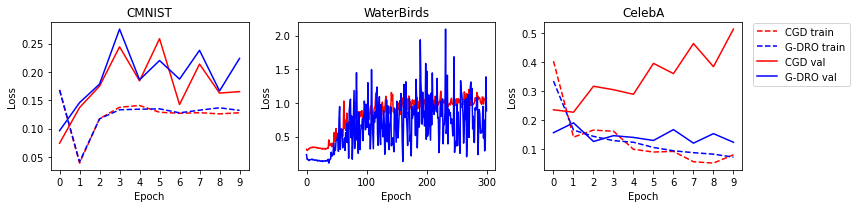
\includegraphics[width=\textwidth]{media/loss-plot-camera-ready.png}
    \centering
    \caption{Loss curves for \texttt{CGD} and \texttt{Group-DRO} on three non-WILDS datasets.}
    \label{fig:monotonicity}
\end{figure}

\section{Discussion}

Overall, the majority of the claims in the paper were reproducible. \texttt{CGD} indeed performed comparably or better than \texttt{ERM} and \texttt{Group-DRO} depending on the dataset. However, the increased runtime of \texttt{CGD} might outweigh the minor accuracy gain. The claim of the authors about the monotonicity of \texttt{CGD} could not be reproduced empirically in a reliable way, and further research is needed. Lastly, \texttt{CGD} appears to have a more stable training in comparison to \texttt{Group-DRO}.

\subsection{What was easy}

The methods used in the paper and the results were described clearly and intuitively. Moreover, the code for \texttt{CGD} was published by the authors alongside clear instructions on integrating it into the WILDS framework. Finally, the framework chosen by the authors is modular, and additional datasets and algorithms could be easily integrated.

\subsection{What was difficult}

\begin{itemize}
    \item \textbf{Resources}: Model training required a massive amount of GPU time due to the dataset size and the sheer number of experiments.
    \item \textbf{Code}: The $C$ parameter for the WILDS implementation of \texttt{Group-DRO} could not be located in the code, so we could not select a value for it. We suspect that there might be an inconsistency between the theory and the code.Even though the code for \texttt{CGD} and WILDS was available, we could not run experiments out of the box: the \texttt{CDG} code had to be updated to work with the latest version of WILDS and required some modifications. Moreover, the dataset code for MultiNLI was missing, so we implemented it following \cite{sagawa2020distributionally} and the advice of the authors.
    \item \textbf{Hyperparameters}: Collecting the correct hyperparameter values was challenging because the paper only provided a range, and there were multiple conflicting sources: the paper, the repository, and the WILDS leaderboard (the latter suggested by the authors in our correspondence). Moreover, some values did not lead to the expected accuracy according to the paper, so we had to experiment with additional values, e.g., the weight decay for CMNIST and Waterbirds. Finally, The best values for the \texttt{CGD} step size $\eta$ in the WILDS leaderboard (0.05 and 0.2) were not in the range described in the paper.
\end{itemize}


\subsection{Communication with original authors}

We reached out to the original authors to obtain more information about the chosen hyperparameter values. They promptly replied, specifying that for the WILDS datasets, the hyperparameters are as configured by default in WILDS 1.2.2. For their algorithm, \texttt{CGD}, they informed us that its hyperparameters could be found in the WILDS leaderboard. In addition, they gave us helpful information about some parts of their code that were missing, such as the MultiNLI dataset.

\newpage